%% packages
\usepackage[centertags,sumlimits,intlimits,namelimits,reqno]{amsmath}
\usepackage{latexsym,amsfonts,amssymb,exscale,enumerate,amsthm,breakcites}
\usepackage[colorlinks,linkcolor=darkblue,citecolor=darkblue,urlcolor=darkblue,breaklinks=true,pagebackref]{hyperref}
\usepackage{tikz}
\usepackage{float,color,multirow,array,multicol}
\usepackage[all,cmtip,2cell]{xy}
\usepackage{fancyhdr}

\usepackage{stmaryrd,mathrsfs}
\usepackage{anyfontsize}


%% headers
\fancyfoot{}
\fancyhead[RO,LE]{\thepage}
\fancyhead[LO]{\textsc\rightmark}
\fancyhead[RE]{\textsc\leftmark}
\renewcommand{\headrulewidth}{0.5pt}

%% chapter titles

%% citations
\definecolor{darkblue}{rgb}{0,0,0.7} 
\renewcommand*{\backref}[1]{(Referred to on page #1.)}

%% theorem environments

\newtheorem{theorem}{Theorem}[chapter]
\newtheorem{lemma}[theorem]{Lemma}
\newtheorem{proposition}[theorem]{Proposition}
\newtheorem{corollary}[theorem]{Corollary}

\newtheorem{conjecture}[theorem]{Conjecture}
%%\renewcommand{\theconj}{\Alph{conjecture}}  % numbered A, B, C etc
%
\theoremstyle{definition}
\newtheorem{definition}[theorem]{Definition}
%\newtheorem{defns}[theorem]{Definitions}
%
%\theoremstyle{remark} 
\newtheorem{example}[theorem]{Example}
\newtheorem{examples}[theorem]{Examples}
%\newtheorem{question}[theorem]{Question}
\newtheorem{remark}[theorem]{Remark}
\newtheorem{notation}[theorem]{Notation}

%% 
\newcommand\maps{{\colon}}
\newcommand{\define}[1]{{\bf \boldmath #1}}

%% tables
\renewcommand{\arraystretch}{1.25}

%% from masters thesis
  \renewcommand{\c}{{\mathcal{C}}}
  \newcommand{\inv}{^{-1}}
  \newcommand{\rr}{{\mathbb{R}}}

%% from decorated cospans

  \newcommand{\R}{{\mathbb{R}}}
  \newcommand{\hooklongrightarrow}{\lhook\joinrel\longrightarrow}
  \newcommand{\linsub}{\operatorname{LinSub}}
  \newcommand{\lgraph}{\operatorname{Graph}}
  \newcommand{\res}{\operatorname{Res}}
  \newcommand{\FinSet}{\mathrm{FinSet}}
  \newcommand{\Set}{\mathrm{Set}}
  \newcommand{\opp}{\mathrm{opp}}

%% from decorated corelations
  \newcommand{\FinVect}{\mathrm{FinVect}}
  \newcommand{\Vect}{\mathrm{Vect}}
  \newcommand{\LinRel}{\mathrm{LinRel}}
  \DeclareMathOperator\corel{{Corel}}
  \DeclareMathOperator\cospan{{Cospan}}


%% from sigflow
\SetSymbolFont{stmry}{bold}{U}{stmry}{m}{n}


\newcommand\z{{\mathbb Z}}
\renewcommand\k{\mathsf{k}}   
\newcommand\nn{{\mathbb N}}
\newcommand\bb{{\mathscr B}}
\newcommand{\idn}{\mathrm{id}}
\newcommand{\tw}{\mathrm{tw}}
\newcommand{\tm}{\tau}
\newcommand\pr{{\R[s,s^{-1}]}}
\newcommand\pk{{\k[s,s^{-1}]}}
\newcommand\pkhom[1]{{\k^{#1}[s,s^{-1}]}}
\newcommand{\Defeq}{\stackrel{\mathrm{def}}{=}}
\newcommand{\vectfun}{\theta}
\newcommand{\cospanfun}{\Theta}
\newcommand{\cospanfunrest}{\overline{\Theta}}
\newcommand{\ha}{\mathbb{HA}}
\newcommand{\ih}{\mathbb{IH}}
\newcommand{\ihcsp}{\ih^{\mathsf{Csp}}}
\newcommand{\ihcor}{\ih^{\mathsf{Cor}}}
\DeclareMathOperator{\mat}{\mathsf{Mat}}
\DeclareMathOperator{\vect}{\mathsf{Vect}}
\DeclareMathOperator{\ltids}{\mathsf{LTI}}
\DeclareMathOperator{\Span}{\mathsf{Span}}
\DeclareMathOperator{\rel}{\mathsf{Rel}}
\DeclareMathOperator{\linrel}{\mathsf{LinRel}}
\DeclareMathOperator{\fmod}{\mathsf{FMod}}
\DeclareMathOperator{\op}{op}
\DeclareMathOperator{\bit}{bit}

\newcommand\addgen{\lower8pt\hbox{$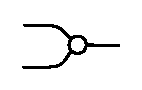
\includegraphics[height=0.7cm]{pics/add.pdf}$}}
\newcommand\zerogen{\lower5pt\hbox{$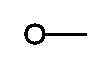
\includegraphics[height=0.5cm]{pics/zero.pdf}$}}
\newcommand\copygen{\lower8pt\hbox{$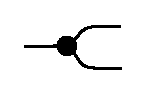
\includegraphics[height=0.7cm]{pics/copy.pdf}$}}
\newcommand\discardgen{\lower5pt\hbox{$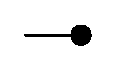
\includegraphics[height=0.5cm]{pics/discard.pdf}$}}
\newcommand\delaygen{\lower6pt\hbox{$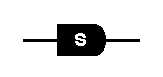
\includegraphics[height=0.6cm]{pics/delay.pdf}$}}
\newcommand\minonegen{\lower6pt\hbox{$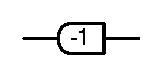
\includegraphics[height=0.6cm]{pics/minone.pdf}$}}
\newcommand\delayopgen{\lower6pt\hbox{$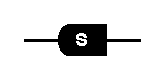
\includegraphics[height=0.6cm]{pics/delayop.pdf}$}}
\newcommand\scalargen{\lower6pt\hbox{$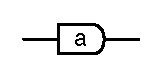
\includegraphics[height=0.6cm]{pics/scalar.pdf}$}}
\newcommand\addopgen{\lower8pt\hbox{$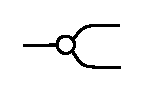
\includegraphics[height=0.7cm]{pics/addop.pdf}$}}
\newcommand\zeroopgen{\lower5pt\hbox{$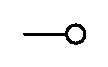
\includegraphics[height=0.5cm]{pics/zeroop.pdf}$}}
\newcommand\copyopgen{\lower8pt\hbox{$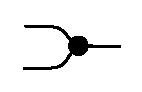
\includegraphics[height=0.7cm]{pics/copyop.pdf}$}}
\newcommand\discardopgen{\lower5pt\hbox{$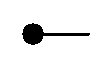
\includegraphics[height=0.5cm]{pics/discardop.pdf}$}}
\newcommand\scalaropgen{\lower6pt\hbox{$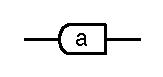
\includegraphics[height=0.6cm]{pics/scalarop.pdf}$}}
\newcommand\delaygenl{\lower6pt\hbox{$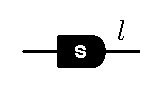
\includegraphics[height=0.6cm]{pics/delayl.pdf}$}}
\newcommand\delayopgenl{\lower6pt\hbox{$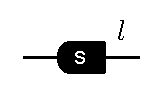
\includegraphics[height=0.6cm]{pics/delayopl.pdf}$}}
\newcommand\delaygenk{\lower6pt\hbox{$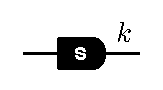
\includegraphics[height=0.6cm]{pics/delayk.pdf}$}}
\newcommand\delayopgenk{\lower6pt\hbox{$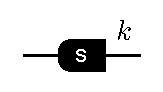
\includegraphics[height=0.6cm]{pics/delayopk.pdf}$}}
\newcommand\twist{\lower6pt\hbox{$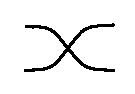
\includegraphics[height=0.6cm]{pics/twist.pdf}$}}
\newcommand\id{\lower3pt\hbox{$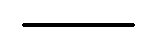
\includegraphics[height=0.3cm]{pics/id.pdf}$}}
\newcommand\syntax{\mathbb{S}}
  

%% from circuits

\newcommand\Z{{\mathbb Z}}   
\newcommand\C{{\mathbb C}}
\newcommand\F{{\mathbb F}}
\newcommand{\vectf}[1]{{\F^{#1} \oplus {(\F^{#1})}^\ast}}
\renewcommand{\twoheadrightarrow}{\to \hspace{-8pt} \to}
\newcommand{\mc}{\mathcal}
\renewcommand{\a}{\alpha}
\newcommand{\s}{\sigma}
\newcommand{\ot}{\otimes}
\newcommand{\eps}{\epsilon}
\newcommand{\ob}{\mathrm{Ob}}
\newcommand{\im}{\mathrm{Im}\,}
\newcommand{\re}{\mathrm{Re}\,}
\newcommand{\mor}{\mathrm{Mor}}
\newcommand{\fgraph}{\operatorname{\mathbb{F}-Graph}}
\newcommand{\Circ}{\mathrm{Circ}}
\newcommand{\LagrRel}{\mathrm{LagrRel}}


